% This file was converted to LaTeX by Writer2LaTeX ver. 1.0.2
% see http://writer2latex.sourceforge.net for more info



\documentclass[twoside,letterpaper]{article}
\usepackage{lscape} %added by Noel
\usepackage[latin1]{inputenc}
\usepackage[T1]{fontenc}
\usepackage[english]{babel}
\usepackage{amsmath}
\usepackage{amssymb,amsfonts,textcomp}
\usepackage{color}
\usepackage{array}
\usepackage{supertabular}
\usepackage{hhline}
\usepackage{hyperref}
\hypersetup{pdftex, colorlinks=true, linkcolor=blue, citecolor=blue, filecolor=blue, urlcolor=blue, pdftitle=SYSTEMS AND SOFTWARE REQUIREMENTS SPECIFICATION (SSRS) TEMPLATE, pdfauthor=Clinton Jeffery, pdfsubject=, pdfkeywords=}
\usepackage[pdftex]{graphicx}

% multiline comment package
\usepackage{verbatim}

% Outline numbering
\setcounter{secnumdepth}{5}
\renewcommand\thesection{\arabic{section}}
\renewcommand\thesubsection{\arabic{section}.\arabic{subsection}}
\renewcommand\thesubsubsection{\arabic{section}.\arabic{subsection}.\arabic{subsubsection}}
\renewcommand\theparagraph{\arabic{section}.\arabic{subsection}.\arabic{subsubsection}.\arabic{paragraph}}
\renewcommand\thesubparagraph{\arabic{section}.\arabic{subsection}.\arabic{subsubsection}.\arabic{paragraph}.\arabic{subparagraph}}
\makeatletter
\newcommand\arraybslash{\let\\\@arraycr}
\makeatother
% Page layout (geometry)
\setlength\voffset{-1in}
\setlength\hoffset{-1in}
\setlength\topmargin{0.5in}
\setlength\oddsidemargin{1in}
\setlength\evensidemargin{1in}
\setlength\textheight{8.278in}
\setlength\textwidth{6.5in}
\setlength\footskip{0.561in}
\setlength\headheight{0.5in}
\setlength\headsep{0.461in}
% Footnote rule
\setlength{\skip\footins}{0.0469in}
\renewcommand\footnoterule{\vspace*{-0.0071in}\setlength\leftskip{0pt}\setlength\rightskip{0pt plus 1fil}\noindent\textcolor{black}{\rule{0.25\columnwidth}{0.0071in}}\vspace*{0.0398in}}
% Pages styles
\makeatletter
\newcommand\ps@Standard{
  \renewcommand\@oddhead{\selectlanguage{english}\rmfamily\color{black} University of Idaho CS Department Instructional Use\hfill \hfill NOT FOR RELEASE}
  \renewcommand\@evenhead{\@oddhead}
  \renewcommand\@oddfoot{\foreignlanguage{english}{\textcolor{black}{SSRS Page }}\foreignlanguage{english}{\textcolor{black}{\thepage{}}}}
  \renewcommand\@evenfoot{\@oddfoot}
  \renewcommand\thepage{\arabic{page}}
}
\newcommand\ps@Convertviii{
  \renewcommand\@oddhead{}
  \renewcommand\@evenhead{\@oddhead}
  \renewcommand\@oddfoot{}
  \renewcommand\@evenfoot{\@oddfoot}
  \renewcommand\thepage{\arabic{page}}
}
\newcommand\ps@Convertvii{
  \renewcommand\@oddhead{}
  \renewcommand\@evenhead{\@oddhead}
  \renewcommand\@oddfoot{}
  \renewcommand\@evenfoot{\@oddfoot}
  \renewcommand\thepage{\arabic{page}}
}
\newcommand\ps@Convertvi{
  \renewcommand\@oddhead{}
  \renewcommand\@evenhead{\@oddhead}
  \renewcommand\@oddfoot{}
  \renewcommand\@evenfoot{\@oddfoot}
  \renewcommand\thepage{\arabic{page}}
}
\newcommand\ps@Convertv{
  \renewcommand\@oddhead{}
  \renewcommand\@evenhead{\@oddhead}
  \renewcommand\@oddfoot{}
  \renewcommand\@evenfoot{\@oddfoot}
  \renewcommand\thepage{\arabic{page}}
}
\newcommand\ps@Convertiv{
  \renewcommand\@oddhead{}
  \renewcommand\@evenhead{\@oddhead}
  \renewcommand\@oddfoot{}
  \renewcommand\@evenfoot{\@oddfoot}
  \renewcommand\thepage{\arabic{page}}
}
\newcommand\ps@Convertii{
  \renewcommand\@oddhead{}
  \renewcommand\@evenhead{\@oddhead}
  \renewcommand\@oddfoot{}
  \renewcommand\@evenfoot{\@oddfoot}
  \renewcommand\thepage{\arabic{page}}
}
\newcommand\ps@FirstPage{
  \renewcommand\@oddhead{}
  \renewcommand\@evenhead{\@oddhead}
  \renewcommand\@oddfoot{}
  \renewcommand\@evenfoot{\@oddfoot}
  \renewcommand\thepage{\arabic{page}}
}
\makeatother
\pagestyle{Standard}
\setlength\tabcolsep{1mm}
\renewcommand\arraystretch{1.3}
% footnotes configuration
\makeatletter
\renewcommand\thefootnote{\arabic{footnote}}
\makeatother
\title{SYSTEMS AND SOFTWARE REQUIREMENTS SPECIFICATION (SSRS) TEMPLATE}
\author{Clinton Jeffery}
\date{2010-11-18T11:33:37.30}
\begin{document}
\clearpage\setcounter{page}{1}\pagestyle{Standard}
\thispagestyle{FirstPage}

\bigskip
%% %% %% %% %% %% %% %% %% %% %% %% %% %% %% %% %% %% %% %% %% %% %% %% %% %% %% %% %% %% 
\begin{comment}
{\centering\selectlanguage{english}\bfseries\color{black}
SYSTEMS AND SOFTWARE REQUIREMENTS SPECIFICATION (SSRS) TEMPLATE
\par}


\bigskip

{\centering\selectlanguage{english}\bfseries\color{black}
Version A.2, September 2010
\par}


\bigskip

{\centering\selectlanguage{english}\bfseries\color{black}
FOREWORD
\par}


\bigskip

{\selectlanguage{english}\color{black}
This document was written to provide software development projects with
a template for generating a System and Software Requirements
Specification (SSRS). \ This document is based on a template originally
written by the U.S. Navy Research, Development, Test and Evaluation
Division in June 1997 in accordance with the MIL-STD-498 DID
(DI-IPSC-81433). \ The template was updated by the University of
Idaho{\textquoteright}s Center for Secure and Dependable Systems (CSDS)
in June 2008 to adhere to IEEE Std. 830-1998, \textit{IEEE Recommended
Practice for Software Requirements
Specifications}\footnote{\foreignlanguage{english}{\ \ \ IEEE Std.
830-1998, }\foreignlanguage{english}{\textit{Recommended Practice for
Software Requirements Specifications}}\foreignlanguage{english}{,
Institute of Electrical and Electronics Engineers, 345 East
47}\foreignlanguage{english}{\textsuperscript{th}}\foreignlanguage{english}{
St. New York, NY, USA, 10017-2394.}}, and IEEE Std. 12207-2008,
\textit{Systems and Software Engineering -- Software Life Cycle
Processes}\footnote{\foreignlanguage{english}{ISO/IEC 12207, IEEE Std.
12207-2008, }\foreignlanguage{english}{\textit{Systems and software
engineering -- Software life cycle
processes}}\foreignlanguage{english}{,
2}\foreignlanguage{english}{\textsuperscript{nd}}\foreignlanguage{english}{
ed., Institute of Electrical and Electronics Engineers, 445 Hoes Lane,
Piscataway, NJ, USA, 08854.}}. It was then adapted in September 2008
for use in UI CS 383.}


\bigskip

{\selectlanguage{english}\color{black}
The SSRS template begins on the next page. \ Just throw away this page
and enter your project specifications into the following template.
\ Don{\textquoteright}t forget to change the headers and footers as
necessary.}


\bigskip


\bigskip



\bigskip




\bigskip




\bigskip


\bigskip

\end{comment}
%% %% %% %% %% %% %% %% %% %% %% %% %% %% %% %% %% %% %% %% %% %% %% %% %% %% %% %% %% %% 
\clearpage{\centering\selectlanguage{english}\bfseries\color{black}
SYSTEMS AND SOFTWARE \ REQUIREMENTS SPECIFICATION (SSRS) FOR 
\par}


\bigskip

{\centering\selectlanguage{english}\bfseries\color{black}
PUML : Project UML
\par}


\bigskip


\bigskip


\bigskip

{\centering\selectlanguage{english}\bfseries\color{black}

\par}

\begin{figure}
\centering

\includegraphics[scale = 3]{viking.png}
\end{figure}

\bigskip


\bigskip

{\centering\selectlanguage{english}\bfseries\color{black}
Version [1.1]
\par}

{\centering\selectlanguage{english}\bfseries\color{black}
[12/16/2011]
\par}


\bigskip


\bigskip

{\centering\selectlanguage{english}\bfseries\color{black}
Prepared for:
\par}

{\centering\selectlanguage{english}\bfseries\color{black}
Bruce Bolden, Dr. Clinton Jeffery
\par}
%{\centering\selectlanguage{english}\bfseries\color{black}
%University of Idaho
%\par}
%{\centering\selectlanguage{english}\bfseries\color{black}
%Moscow, ID \ 83844-1010
%\par}

\bigskip

\bigskip

{\centering\selectlanguage{english}\bfseries\color{black}
Prepared by:
\par}

{\centering\selectlanguage{english}\bfseries\color{black}
Coleman Beasley, Alex Dean, Austin Enfield, Jason Fletcher, Theora Rice, Cable Johnson, Adrian Norris, David Summers
\par}

\bigskip

{\centering\selectlanguage{english}\bfseries\color{black}
Emeritus Contributors:
\par}

{\centering\selectlanguage{english}\bfseries\color{black}
Noel Klein, Max McKinnon
\par}

\bigskip
\bigskip

{\centering\selectlanguage{english}\bfseries\color{black}
University of Idaho
\par}

{\centering\selectlanguage{english}\bfseries\color{black}
Moscow, ID \ 83844-1010
\par}

\clearpage{\centering\selectlanguage{english}\bfseries\color{black}
PUML SSRS
\par}


\bigskip

{\centering\selectlanguage{english}\bfseries\color{black}
RECORD OF CHANGES (N/A)
\par}


\bigskip

\begin{flushleft}
\tablehead{}
\begin{supertabular}{|m{0.47685984in}|m{0.6087598in}|m{1.3587599in}|m{0.23375985in}|m{2.0462599in}|m{0.7337598in}|m{0.6330598in}|}
\hline
~

\centering \selectlanguage{english}\color{black} Change number &
~

\centering \selectlanguage{english}\color{black} Date completed &
~

\centering \selectlanguage{english}\color{black} Location of change
(e.g., page or figure \#) &
\centering \selectlanguage{english}\bfseries\color{black} A\newline
M\newline
D &
~

~

\centering \selectlanguage{english}\color{black} Brief description of
change &
~

\centering \selectlanguage{english}\color{black} Approved by (initials)
&
~

\centering\arraybslash \selectlanguage{english}\color{black} Date
Approved\\\hline
1
 &
2012.02.05
 &
cover sheet
 &
M
 &
Added Dr. Jeffery to "prepared for", modified version. Per lecture 9.
 &
DS
 &

\\\hline
~
 &
~
 &
~
 &
~
 &
~
 &
~
 &
~
\\\hline
~
 &
~
 &
~
 &
~
 &
~
 &
~
 &
~
\\\hline
~
 &
~
 &
~
 &
~
 &
~
 &
~
 &
~
\\\hline
~
 &
~
 &
~
 &
~
 &
~
 &
~
 &
~
\\\hline
~
 &
~
 &
~
 &
~
 &
~
 &
~
 &
~
\\\hline
~
 &
~
 &
~
 &
~
 &
~
 &
~
 &
~
\\\hline
~
 &
~
 &
~
 &
~
 &
~
 &
~
 &
~
\\\hline
~
 &
~
 &
~
 &
~
 &
~
 &
~
 &
~
\\\hline
~
 &
~
 &
~
 &
~
 &
~
 &
~
 &
~
\\\hline
~
 &
~
 &
~
 &
~
 &
~
 &
~
 &
~
\\\hline
~
 &
~
 &
~
 &
~
 &
~
 &
~
 &
~
\\\hline
~
 &
~
 &
~
 &
~
 &
~
 &
~
 &
~
\\\hline
~
 &
~
 &
~
 &
~
 &
~
 &
~
 &
~
\\\hline
~
 &
~
 &
~
 &
~
 &
~
 &
~
 &
~
\\\hline
~
 &
~
 &
~
 &
~
 &
~
 &
~
 &
~
\\\hline
~
 &
~
 &
~
 &
~
 &
~
 &
~
 &
~
\\\hline
~
 &
~
 &
~
 &
~
 &
~
 &
~
 &
~
\\\hline
~
 &
~
 &
~
 &
~
 &
~
 &
~
 &
~
\\\hline
~
 &
~
 &
~
 &
~
 &
~
 &
~
 &
~
\\\hline
~
 &
~
 &
~
 &
~
 &
~
 &
~
 &
~
\\\hline
~
 &
~
 &
~
 &
~
 &
~
 &
~
 &
~
\\\hline
~
 &
~
 &
~
 &
~
 &
~
 &
~
 &
~
\\\hline
~
 &
~
 &
~
 &
~
 &
~
 &
~
 &
~
\\\hline
\end{supertabular}
\end{flushleft}
{\selectlanguage{english}\color{black}
\foreignlanguage{english}{*}\foreignlanguage{english}{\textbf{A}}\foreignlanguage{english}{
- ADDED
\ }\foreignlanguage{english}{\textbf{M}}\foreignlanguage{english}{ -
MODIFIED
\ }\foreignlanguage{english}{\textbf{D}}\foreignlanguage{english}{ -
DELETED}}

\clearpage{\centering\selectlanguage{english}\bfseries\color{black}
\foreignlanguage{english}{\MakeUppercase{\ }}\foreignlanguage{english}{\MakeUppercase{PUML SSRS}}
\par}

{\centering\selectlanguage{english}\bfseries\color{black}
TABLE OF CONTENTS
\par}


\bigskip

{\selectlanguage{english}\bfseries\color{black}
Section\ \ Page}

\setcounter{tocdepth}{9}
\renewcommand\contentsname{}
\tableofcontents

\bigskip

\clearpage\clearpage\setcounter{page}{1}\pagestyle{Convertii}
\section[Introduction (Alex)]{\selectlanguage{english}\rmfamily\bfseries\color{black}
Introduction (Alex)}
{\selectlanguage{english}\color{black}


\subsection[IDENTIFICATION]{\selectlanguage{english}\rmfamily\bfseries\color{black}
IDENTIFICATION}


{\selectlanguage{english}\color{black}
	The software system being considered for development is referred to as pUML.	The customer providing specifications for the system is Bruce Bolden. The ultimate customer, or end-user, of the system will be Bruce Bolden and his associates. This is a new project effort, so the version under development is version 1.0.
}

\subsection[PURPOSE]{\selectlanguage{english}\rmfamily\bfseries\color{black}
PURPOSE}


{\selectlanguage{english}\color{black}
	The purpose of the system under development is to develop a flexible and easy to use UML diagram editor.	While the system will be used by Bruce Bolden and his associates, this document is intended to be read and understood by UICS software designers and coders.}

\subsection[SCOPE]{\selectlanguage{english}\rmfamily\bfseries\color{black}
SCOPE}

{\selectlanguage{english}\color{black}
	The system being developed was started on October 12th, 2011.  The project sponsor and user is Bruce Bolden.  The developers are Coleman Beasley, Alex Dean, Jason Fletcher, Noel Klein, Max McKinnon, and Theora Rice.}

\subsection[DEFINITIONS, ACRONYMS, AND
ABBREVIATIONS]{\selectlanguage{english}\rmfamily\bfseries\color{black}
DEFINITIONS, ACRONYMS, AND ABBREVIATIONS}

\bigskip

\begin{flushleft}
\tablehead{}
\begin{supertabular}{|m{1.3587599in}|m{5.00806in}|}
\hline
\centering \selectlanguage{english}\bfseries\color{black} Term or
Acronym &
\centering\arraybslash \selectlanguage{english}\bfseries\color{black}
Definition\\\hline
\selectlanguage{english}\color{black} Alpha test &
\selectlanguage{english}\color{black} Limited release(s) to selected,
outside testers\\\hline
\selectlanguage{english}\color{black} Beta test &
\selectlanguage{english}\color{black} Limited release(s) to cooperating
customers wanting early access to developing systems\\\hline
\selectlanguage{english}\color{black} Final test &
\selectlanguage{english}\color{black} aka, Acceptance test, release of
full functionality to customer for approval\\\hline
\selectlanguage{english}\color{black} DFD &
\selectlanguage{english}\color{black} Data Flow Diagram\\\hline
\selectlanguage{english}\color{black} SDD &
\selectlanguage{english}\color{black} Software Design Document, aka SDS,
Software Design Specification\\\hline
\selectlanguage{english}\color{black} SRS &
\selectlanguage{english}\color{black} Software Requirements
Specification\\\hline
\selectlanguage{english}\color{black} SSRS &
\selectlanguage{english}\color{black} System and Software Requirements
Specification\\\hline
~
 &
~
\\\hline
~
 &
~
\\\hline
~
 &
~
\\\hline
~
 &
~
\\\hline
\end{supertabular}
\end{flushleft}
\subsection[REFERENCES]{\selectlanguage{english}\rmfamily\bfseries\color{black}
REFERENCES}
	

{\selectlanguage{english}\itshape\color{black}
{Qt - drag and drop with graphics view framework} }{\selectlanguage{english}\color{black} Internet. Available: http://stackoverflow.com/questions/2732343/qt-drag-and-drop-with-graphics-view-framework}


\subsection[OVERVIEW AND
RESTRICTIONS]{\selectlanguage{english}\rmfamily\bfseries\color{black}
OVERVIEW AND RESTRICTIONS}

{\selectlanguage{english}\color{black}
	This document is for limited release only to UI CS personnel working on the project.}


\bigskip

{\selectlanguage{english}\color{black}
Section 2 of this document describes the system under development from a
holistic point of view. \ Functions, characteristics, constraints,
assumptions, dependencies, and overall requirements are defined from
the system-level perspective.}


\bigskip

{\selectlanguage{english}\color{black}
Section 3 of this document describes the specific requirements of the
system being developed. \ Interfaces, features, and specific
requirements are enumerated and described to a degree sufficient for a
knowledgeable designer or coder to begin crafting an architectural
solution to the proposed system.}


\bigskip

{\selectlanguage{english}\color{black}
Section 4 provides the requirements traceability information for the
project. \ Each feature of the system is indexed by the SSRS
requirement number and linked to its SDD and test references.}


\bigskip

{\selectlanguage{english}\color{black}
Sections 5 and up are appendices including original information and
communications used to create this document.}

%Section written by Coleman Beasley 
\section[OVERALL DESCRIPTION (CKB)]{\selectlanguage{english}\rmfamily\bfseries\color{black}
OVERALL DESCRIPTION (Coleman)}


\subsection[PRODUCT PERSPECTIVE]{\selectlanguage{english}\rmfamily\bfseries\color{black}
PRODUCT PERSPECTIVE}

{\selectlanguage{english}\color{black}
This software is completely independent and self-contained.}

\subsection[PRODUCT
FUNCTIONS]{\selectlanguage{english}\rmfamily\bfseries\color{black}
PRODUCT FUNCTIONS}

{\selectlanguage{english}\color{black}
Our product is a Unified Modeling Language (UML) diagram editor.
It creates 5 different types of diagrams and exports them into user-friendly formats. The editor streamlines the creation process by making available only shapes that apply to the current diagram. Multiple shape and line colors are supported to allow for more versatile diagrams.}

\subsection[USER
CHARACTERISTICS]{\selectlanguage{english}\rmfamily\bfseries\color{black}
USER CHARACTERISTICS}

{\selectlanguage{english}\color{black}
The users of the product will be software developers who are in the planning phases of their project. Users are expected to be familiar with UML diagrams and understand the basic idea behind each drawing. The software will attempt to make the process easier, but a basic understanding will be necessary to use  the editor effectively.}

\subsection[CONSTRAINTS]
{\selectlanguage{english}\rmfamily\bfseries\color{black}
CONSTRAINTS}

{\selectlanguage{english}\color{black}
There are no applicable constraints.}

\subsection[ASSUMPTIONS AND
DEPENDENCIES]{\selectlanguage{english}\rmfamily\bfseries\color{black}
ASSUMPTIONS AND DEPENDENCIES}


{\selectlanguage{english}\color{black}
The software is built with the assumption that the hardware and operating system it is installed on will support the Qt graphics library.}

\subsection[SYSTEM LEVEL (NON-FUNCTIONAL)
REQUIREMENTS]
{\selectlanguage{english}\rmfamily\bfseries\color{black}
SYSTEM LEVEL (NON-FUNCTIONAL) REQUIREMENTS}


\subsubsection[Site
dependencies]{\selectlanguage{english}\rmfamily\bfseries\color{black}
Site dependencies}

{\selectlanguage{english}\color{black}
There are no anticipated site dependencies.}

\subsubsection[Safety, security and privacy
requirements]{\selectlanguage{english}\rmfamily\bfseries\color{black}
Safety, security and privacy requirements}


{\selectlanguage{english}\color{black}
There are no safety, security or privacy requirements for the system.}

\subsubsection[Performance
requirements]{\selectlanguage{english}\rmfamily\bfseries\color{black}
Performance requirements}

{\selectlanguage{english}\color{black}
The program is intended for use by one user at a time.  There are no other performance requirements.}

\subsubsection[System and software
quality]{\selectlanguage{english}\rmfamily\bfseries\color{black} System
and software quality}


{\selectlanguage{english}\color{black}
The software shall create, edit and save 5 types of UML diagrams.  It is designed to operate in the same general manner for each diagram. The software is designed as modularly as possible to allow for ease of modification. It is designed to be run on as many systems as possible. For this reason, it is being developed in C++ using an open source graphics system.}

\subsubsection[Packaging and delivery
requirements]{\selectlanguage{english}\rmfamily\bfseries\color{black}
Packaging and delivery requirements}


{\selectlanguage{english}\color{black}
The executable system and all associated documentation (i.e., SSRS, SDD,
code listing, test plan (data and results), and user manual) will be
delivered to the customer on CD{\textquoteright}s and/or via email, as
specified by the customer at time of delivery. \ Although document
{\textquotedblleft}drops{\textquotedblright} will occur throughout the
system development process, the final, edited version of the above
documents will accompany the final, accepted version of the executable
system.}

\subsubsection[Personnel-related
requirements]
{\selectlanguage{english}\rmfamily\bfseries\color{black}
Personnel-related requirements}


{\selectlanguage{english}\color{black}
The system under development has no special personnel-related
requirements. }

\subsubsection[Training-related
requirements]{\selectlanguage{english}\rmfamily\bfseries\color{black}
Training-related requirements}

{\selectlanguage{english}\color{black}
No training materials or expectations are tied to this project other
than the limited help screens built into the software and the
accompanying user manual.}

\subsubsection[Logistics-related
requirements]{\selectlanguage{english}\rmfamily\bfseries\color{black}
Logistics-related requirements}

{\selectlanguage{english}\color{black}
The system requires a computer that can run Windows, Mac OSX, or Linux (x86 or x64).  The only peripheral hardware needs are a mouse, keyboard, monitor, and printer(optional)}

\subsubsection[Other
requirements]{\selectlanguage{english}\rmfamily\bfseries\color{black}
Other requirements}


{\selectlanguage{english}\color{black}
There are no other requirements.}

\subsubsection[Precedence and criticality of
requirements]{\selectlanguage{english}\rmfamily\bfseries\color{black}
Precedence and criticality of requirements}

{\selectlanguage{english}\color{black}
No requirements have been defined as critical.}
%End of Coleman Beasley's section 

% The following section was edited by noel
\clearpage\section[SPECIFIC
REQUIREMENTS (Noel)]{\selectlanguage{english}\rmfamily\bfseries\color{black}
SPECIFIC REQUIREMENTS (Noel)}
{\selectlanguage{english}\itshape\color{black}
This section of the document contains all of the software
requirements to a level of detail sufficient to enable designers to
design a system to satisfy those requirements, and testers to test that
the system satisfies those requirements. \ Throughout this section,
every stated requirement is externally perceivable by users,
operators, or other external systems. \ All requirements include at a minimum a description of every input \ into the system, every output from the system, and all functions performed by the system
in response to an input or in support of an output.}
%edited

\subsection[EXTERNAL INTERFACE
REQUIREMENTS]{\selectlanguage{english}\rmfamily\bfseries\color{black}
EXTERNAL INTERFACE REQUIREMENTS}
{\selectlanguage{english}\itshape\color{black}
This subsection is a detailed description of all inputs into and
outputs from the software system. \ It complements the
constraints and dependencies defined in earlier sections. \ Hardware, software, user, and other
communication interfaces are specified.}
%edited

\subsubsection[Hardware
Interfaces]{\selectlanguage{english}\rmfamily\bfseries\color{black}
Hardware Interfaces}
{\selectlanguage{english}\color{black}
\foreignlanguage{english}{\ }\foreignlanguage{english}{For the purpose of the UML application, there is no special hardware necessary. Only standard computer interfaces, such as a monitor, a keyboard and a mouse are required. A printer is necessary, if the user wishes to print out the diagrams.}}
%edited

\subsubsection[Software
Interfaces]{\selectlanguage{english}\rmfamily\bfseries\color{black}
Software Interfaces}
{\selectlanguage{english}\color{black}
\foreignlanguage{english}{\ }\foreignlanguage{english}{The customer did not demand any specific software interfaces. There is also no special interface for the development and function necessary. Only the print dialog will connect to the users printer driver software or use the OS's default dialog.}}
%edited

\subsubsection[User
Interfaces]{\selectlanguage{english}\rmfamily\bfseries\color{black}
User Interfaces}
{\selectlanguage{english}\color{black}
\foreignlanguage{english}{\ }\foreignlanguage{english}{The user will be able to use the usual computer input types, such as keyboard and mouse to use the graphical user interface of the UML tool.}}
%edited

\subsubsection[Other Communication
Interfaces]{\selectlanguage{english}\rmfamily\bfseries\color{black}
Other Communication Interfaces}
{\selectlanguage{english}\color{black}
\foreignlanguage{english}{\ }\foreignlanguage{english}{No other communication interfaces are needed.}}
%edited

\bigskip


\bigskip

\bigskip
\begin{landscape}
\clearpage\setcounter{page}{1}

\bigskip

\begin{flushleft}
\tablehead{}
\begin{supertabular}{|m{0.7337598in}|m{1.4212599in}|m{2.7337599in}|m{1.0462599in}|m{1.4837599in}|m{1.1087599in}m{-0.054440156in}|}
\multicolumn{6}{m{8.92126in}}{\centering
{\selectlanguage{english}\bfseries\color{black} External Interface
Requirements}\par

~

\centering \selectlanguage{english}\bfseries\color{black} Hardware
Interfaces} &
\multicolumn{1}{m{-0.054440156in}}{~
}\\\hline
\centering \selectlanguage{english}\bfseries\color{black} Name &
\centering \selectlanguage{english}\bfseries\color{black}
Source/Destination &
\centering \selectlanguage{english}\bfseries\color{black} Description &
\centering \selectlanguage{english}\bfseries\color{black} Type/range &
\centering \selectlanguage{english}\bfseries\color{black} Dependencies &
\multicolumn{2}{m{1.1330599in}|}{\centering
\selectlanguage{english}\bfseries\color{black} Formats}\\\hline
Keyboard
 &
Keyboard/Text fields
 &
Text input
 &
Standard
 &
~
 &
\multicolumn{2}{m{1.1330599in}|}{~
}\\\hline
Mouse
 &
Mouse/GUI
 &
For using the GUI
 &
Standard
 &
~
 &
\multicolumn{2}{m{1.1330599in}|}{~
}\\\hline
Monitor
 &
GUI/Monitor
 &
Display GUI
 &
Standard
 &
~
 &
\multicolumn{2}{m{1.1330599in}|}{~
}\\\hline
Printer
 &
Diagram/Printer
 &
Print diagram
 &
Standard
 &
~
 &
\multicolumn{2}{m{1.1330599in}|}{~
}\\\hline
\multicolumn{6}{m{8.92126in}}{~

\centering \selectlanguage{english}\bfseries\color{black} Software
Interfaces} &
\multicolumn{1}{m{-0.054440156in}}{~
}\\\hline
\centering \selectlanguage{english}\bfseries\color{black} Name &
\centering \selectlanguage{english}\bfseries\color{black}
Source/Destination &
\centering \selectlanguage{english}\bfseries\color{black} Description &
\centering \selectlanguage{english}\bfseries\color{black} Type/range &
\centering \selectlanguage{english}\bfseries\color{black} Dependencies &
\multicolumn{2}{m{1.1330599in}|}{\centering
\selectlanguage{english}\bfseries\color{black} Formats}\\\hline
Print dialog
 &
OS/UML tool
 &
Standard OS printer dialog
 &
~
 &
~
 &
\multicolumn{2}{m{1.1330599in}|}{~
}\\\hline
\multicolumn{6}{m{8.92126in}}{~

\centering \selectlanguage{english}\bfseries\color{black} User
Interfaces} &
\multicolumn{1}{m{-0.054440156in}}{~
}\\\hline
\centering \selectlanguage{english}\bfseries\color{black} Name &
\centering \selectlanguage{english}\bfseries\color{black}
Source/Destination &
\centering \selectlanguage{english}\bfseries\color{black} Description &
\centering \selectlanguage{english}\bfseries\color{black} Type/range &
\centering \selectlanguage{english}\bfseries\color{black} Dependencies &
\multicolumn{2}{m{1.1330599in}|}{\centering
\selectlanguage{english}\bfseries\color{black} Formats}\\\hline
GUI
 &
GUI/Monitor
 &
The UML tool is used via the GUI
 &
~
 &
~
 &
\multicolumn{2}{m{1.1330599in}|}{~
}\\\hline

\end{supertabular}
\end{flushleft}
\end{landscape}
\clearpage\setcounter{page}{1}
\subsection[SYSTEM
FEATURES]{\selectlanguage{english}\rmfamily\bfseries\color{black}
SYSTEM FEATURES}
{\selectlanguage{english}\itshape\color{black}
The functional requirements in this section define the fundamental actions (i.e.,
features) \ that must take place in the UML tool in accepting and
processing the inputs and in processing and generating the outputs.
These requirements are given in the form of \textbf{Use Cases} where
possible, denoting a concrete use (discrete user-performable task) of
the system. Use case diagrams are followed by use case descriptions.}
%edited
\subsubsection[\ Use Case
Diagrams]{\foreignlanguage{english}{\ }\foreignlanguage{english}{Use
Case Diagrams}}
\paragraph*{File operations}
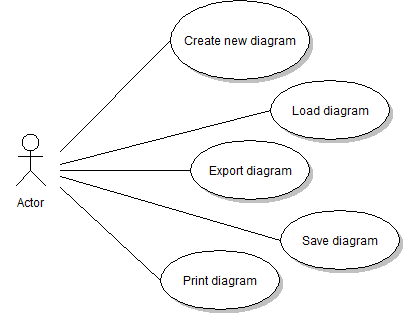
\includegraphics[scale=0.6]{../UMLdiagrams/use_case_files.png}

\paragraph*{Drawing use cases 1}
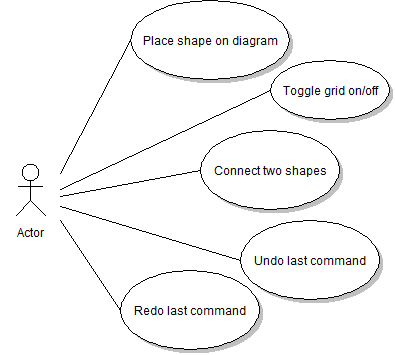
\includegraphics[scale=0.6]{../UMLdiagrams/draw1.png}
\paragraph*{Drawing use cases 2}
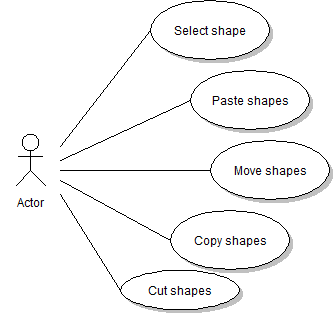
\includegraphics[scale=0.6]{../UMLdiagrams/draw2.png}
\paragraph*{Shape properties}
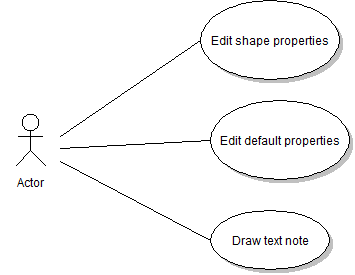
\includegraphics[scale=0.6]{../UMLdiagrams/properties.png}

\bigskip

\subsubsection{Use Case Descriptions}

\paragraph{Create new diagram - Req No. UC1\newline}
 Actors - User
Goals - Create a new diagram\\
Preconditions - UML editor is started\\
Summary - The user creates a new diagram.\\
Related use cases - none\\
Steps\\
1. Click new on the top toolbar. \\
2. A dialogue pops up. Choose the diagram type in the dialogue.\\
3. Click create.\\
Alternatives - none \\
Post conditions - There is an empty diagram.  The diagram specific tools are activated on the left toolbar. One can now start drawing a UML diagram.

\paragraph{Load a diagram - Req No. UC2\newline}
Actors- User\\
Goals- Load a previously saved diagram\\
Preconditions - UML editor is started\\
Summary - The user loads a previously saved diagram from the file system.\\
Related use cases - none\\
Steps\\
1. Click open on the top toolbar.\\
2. A dialog pops up. Navigate through your file system. Choose the file.\\
3. Click open.\\
Alternatives - none\\
Post conditions - The saved diagram is open.  The diagram specific tools are activated on the left toolbar. One can now start editing the UML diagram.\\

\paragraph{Export a diagram - Req No. UC3\newline}
Actors - User\\
Goals - Export the open diagram\\
Preconditions - Diagram file is opened\\
Summary - The user exports the open diagram to a PDF file.\\
Related use cases - none\\
Steps\\
1. Click save on the top toolbar. \\
2. Click export to PDF in the pop-down menu.\\
3. Enter a filename.\\
4. Click save.\\
Alternatives - none\\
Post conditions - The diagram is exported as a PDF file. The PDF file is saved in the user specified location of the users file system.\\

\paragraph{Save a diagram - Req No. UC4\newline}
Actors - User\\
Goals - Save the open diagram\\
Preconditions - Diagram file is opened\\
Summary - The user saves the open diagram to a XML file.\\
Related use cases - none\\
Steps\\
1. Click save on the top toolbar.\\
2. Click save as file in the pop-down menu.\\
3. Enter a filename.\\
4. Click save.\\
Alternatives - none\\
Post conditions - The diagram is saved as an XML file. The XML file is saved in the user specified location of the users file system.\\

\paragraph{Print a diagram - Req No. UC5\newline}
Actors - User\\
Goals - Print the open diagram\\
Preconditions - Diagram file is opened\\
Summary - The user prints the open diagram. The UML tool uses the OS's  print dialog and therefore the OS's print drivers.\\
Related use cases - none\\
Steps\\
1. Click print on the top toolbar.\\
2. Select a printer.\\
3. Select printer specific options. \\
4. When you are satisfied with the settings, click print.\\
Alternatives - none\\
Post conditions - The diagram is printed. \\

\paragraph{Toggle grid on/off - Req No. UC6\newline}
Actors - User\\
Goals - Toggle the grid of the drawing area on or off\\
Preconditions - Diagram file is opened\\
Summary - The user toggles the grid of the drawing area on or off.\\
Related use cases - none\\
Steps\\
1. Click on grid on the top toolbar.\\
Alternatives - none\\
Post conditions - If the grid was turned on, the grid is turned off. If the grid was turned off, the grid is turned on.\\

\paragraph{Place shapes on diagram - Req No. UC7\newline}
Actors - User\\
Goals - Place a shape on the drawing area\\
Preconditions - Diagram file is opened\\
Summary - The user chooses a shape from the drawing toolbar and places it on the drawing area.\\
Related use cases - none \\
Steps\\
1. Select the shape from the left drawing toolbar.\\
2. Click on the diagram to place the shape on the diagram.\\
Alternatives - none\\
Post conditions - The selected shape is placed on the drawing area at the place pointed at by the user.\\

\paragraph{Connect shapes - Req No. UC8\newline}
Actors - User\\
Goals - Connect two shapes on the drawing area with a connecting line\\
Preconditions - Diagram file is opened\\
Summary - The user chooses a line type from the drawing toolbar and specifies the two shapes on the drawing area to connect.\\
Related use cases - none\\
Steps\\
1. Select a connector from the left drawing toolbar.\\
2. Click on the source shape.\\
3. Click on the target shape.\\
4. A connecting line is placed from the source shape to the target shape.\\
Alternatives - none\\
Post conditions - The selected line connects is placed on the drawing area at the place pointed at by the user.\\

\paragraph{Undo commands - Req No. UC9\newline}
Actors - User\\
Goals - Undo the last command\\
Preconditions - Diagram file is opened. A command has been used.\\
Summary - The last action taken by the user is being undone and put into a redo stack.\\
Related use cases - none\\
Steps\\
1. Click undo on the top toolbar.\\
2. The last command is revoked.\\
3. Continue drawing.\\
Alternatives - none\\
Post conditions - The last command is revoked and stored in the redo.\\

\paragraph{Redo commands - Req No. UC10\newline}
Actors - User\\
Goals - Redo the last undone command\\
Preconditions - Diagram file is opened. A command has been undone.\\
Summary - The last action on top of the redo stack is redone and removed from the stack.\\
Related use cases - none\\
Steps\\
1. Click redo on the top toolbar.\\
2. The last revoked command is redone.\\
3. Continue drawing.\\
Alternatives - none\\
Post conditions - The last undone action is redone and removed from the stack.\\

\paragraph{Select shapes and multiple shapes - Req No. UC11\newline}
Actors - User\\
Goals - Select one or more shapes\\
Preconditions - Shapes are available to select on the drawing area. \\
Summary - The user selects the shapes for further commands.\\
Related use cases - none\\
Steps//
1. Click on a shape to select it.\\
2. Hold CTRL and click other shapes to select multiple shapes.\\
Alternatives - none\\
Post conditions - The selected shapes are marked. Further commands can be invoked to all selected shapes.\\

\paragraph{Move shapes - Req No. UC12\newline}
Actors - User\\
Goals - Move one or more shapes\\
Preconditions - One or more shapes are selected\\
Summary - The user moves the shapes to a different location on the drawing area.\\
Related use cases - none\\
Steps\\
1. Select one or more shapes.\\
2. Click and hold the mouse button on one of the shapes.\\
3. Move the shapes to a new place.\\
4. Release the mouse button\\
Alternatives - none\\
Post conditions - The selected shapes are moved to the new place.\\

\paragraph{Copy shapes - Req No. UC13\newline}
Actors - User\\
Goals - Copy one or more shapes\\
Preconditions - One or more shapes are selected\\
Summary - The user copies the selected shapes to the clipboard.\\
Related use cases - none\\
Steps\\
1. Select one or more shapes.\\
2. Click copy on the top toolbar.\\
Alternatives - none\\
Post conditions - The selected shapes are copied to the clipboard and can be pasted in a drawing area.\\

\paragraph{Cut shapes - Req No. UC14\newline}
Actors - User\\
Goals - Cut one or more shapes\\
Preconditions - One or more shapes are selected\\
Summary - The user cuts the selected shapes to the clipboard. The shapes are removed from the drawing area.\\
Related use cases - none\\
Steps\\
1. Select one or more shapes.\\
2. Click cut on the top toolbar.\\
Alternatives - none\\
Post conditions - The selected shapes are copied to the clipboard and can be pasted in a drawing area. The shapes are removed from the drawing area.\\

\paragraph{Paste shapes - Req No. UC15\newline}
Actors - User\\
Goals - Paste one or more shapes\\
Preconditions - A selection of shapes is stored in the clipboard\\
Summary - The user pastes the shapes from the clipboard into the drawing area.\\
Related use cases - none\\
Steps\\
1. Click paste on the top toolbar.\\
Alternatives - none\\
Post conditions - The shapes from the clipboard are inserted in the top left corner of the diagram.\\

\paragraph{Edit shape properties - Req No. UC16\newline}
Actors - User\\
Goals - Change the properties of a single shape\\
Preconditions - A shape is available for editing on the draw area.\\
Summary - The user edits a shape on the drawing area.\\
Related use cases - none\\
Steps\\
1. Select one shape.\\
2. Click shape preferences on the top toolbar.\\
3. Select shape specific options. \\
4. When you are satisfied with the settings, click ok.\\
Alternatives - Instead of selecting a shape and clicking shape preferences on the toolbar, one can also double click on a shape to get to the shape specific options.\\
Post conditions - The shape properties are changed.\\

\paragraph{Edit default properties - Req No. UC17\newline}
Actors - User\\
Goals - Change the default properties of the UML tool\\
Preconditions - UML editor is started\\
Summary - The user edits the default properties of the UML tool.\\
Related use cases - none\\
Steps\\
1. Click on options on the top toolbar.\\
2. Modify preferences for the default shapes.\\
\indent The shape options are:\\
- Color\\
- Fill color\\
- Line thickness\\

\indent The line options are:\\
- Color\\
- Thickness\\

\indent The text options are:\\
- Color\\
- Font\\
- Size\\
- Fill color\\
- Border color\\
Alternatives - none\\
Post conditions - The default properties are changed.\\


% Noel end

% The following section was edited by Noel and Max

\clearpage\setcounter{page}{1}\pagestyle{Convertvi}
\section[REQUIREMENTS
TRACEABILITY (Noel and Max)]{\selectlanguage{english}\rmfamily\bfseries\color{black}
REQUIREMENTS TRACEABILITY (Noel)}

\bigskip
\begin{flushleft}
\tablehead{%
\hline
Feature Name & Req No. & Requirement Description & Priority \\
\hline}
\begin{supertabular}{|m{1.5in}|m{0.6in}|m{3.5in}|m{0.7in}|}
Create a new diagram & UC1 & The user creates a new diagram. & Mandatory
\\\hline
Load a diagram & UC2 & The user loads a previously saved diagram from the file system. & Mandatory
\\\hline
Export a diagram & UC3 & The user exports the open diagram to a PDF file.
Related use cases & low
\\\hline
Save a diagram & UC4 & The user saves the open diagram to a XML file.
Related use cases & Mandatory
\\\hline
Print a diagram & UC5 & The user prints the open diagram. The UML tool uses the OS's  print dialog and therefore the OS's print drivers. & low
\\\hline
Toggle grid on/off & UC6 & The user toggles the grid of the drawing area on or off. & high
\\\hline
Place shapes on diagram & UC7 & The user chooses a shape from the drawing toolbar and places it on the drawing area. & Mandatory
\\\hline
Connect shapes & UC8 & The user chooses a line type from the drawing toolbar and specifies the two shapes on the drawing area to connect. & Mandatory
\\\hline
Undo commands & UC9 & The last action taken by the user is being undone and put into a redo stack. & low
\\\hline
Redo commands & UC10 & The last action on top of the redo stack is redone and removed from the stack. & low
\\\hline
Select shapes & UC11 & The user selects the shapes for further commands. & low
\\\hline
Move shapes & UC12 & The user moves the shapes to a different location on the drawing area. & high
\\\hline
Copy shapes & UC13 & The user copies the selected shapes to the clipboard. & low
\\\hline
Cut shapes & UC14 & The user cuts the selected shapes to the clipboard. The shapes are removed from the drawing area. & low
\\\hline
Paste shapes & UC15 & The user pastes the shapes from the clipboard into the drawing area. & low
\\\hline
Edit shape properties & UC16 & The user edits a shape on the drawing area. & low
\\\hline
Edit default properties & UC17 & The user edits the default properties of the UML tool. & low
\\\hline
\end{supertabular}
\end{flushleft}
{\selectlanguage{english}\color{black}
Priorities are: \textbf{M}andatory, \textbf{L}ow, \textbf{H}igh}

% Noel and Max end

\clearpage\setcounter{page}{1}\pagestyle{Convertvii}
\section[APPENDIX A. \ List of Requirements]{\selectlanguage{english}\rmfamily\bfseries\color{black}
APPENDIX A. \ List of Requirements}

\bigskip

{\selectlanguage{english}\color{black}

\begin{list}{-} %{spacing}
\item Should support the five main types of diagrams
\item Should have a library of UML Graphical Objects
\item File (Open/Close/Save/Import)
\item Easy to use
\item Portable-ish
\item Light on System Resources
\item Cut/Copy/Duplicate/Paste
\item Undo/Redo
\item Keyboard Bindings
\item Template Generation
\item Diagram from code
\item UML syntax parser
\item Print and export to graphics, cover page generation
\item GUI
\item Support for defects
\item Installer
\item Collaborative Support
\item Project Manager (File Organizer)/File Linking
\item Multiple Documents
\item Man page/Help/user manual/tutorials
\item Color
\item Snap to grid/alignment
\item Scaling/zoom
\item Font selection
\item Spell check
\item Change settings
\item Default UML Diagram template
\item Text editor (LaTeX)
\item Tool Tips, in many forms
\item Collapse branches, trees
\item Integrate with other UML editors
\item File Format (internal)
\item XML MUST FORMAT
\item Script to auto-save and create backups
\item Special character support
\item FIND and replace
\end{list}



\bigskip
\end{document}
